\documentclass[12pt,a4paper]{article}
\usepackage{textcomp, gensymb}
\usepackage[italian]{babel}
\usepackage{newlfont}
\usepackage{gensymb}
\usepackage{hyperref}
\usepackage{graphicx}
\usepackage{mathtools}

\textwidth=450pt\oddsidemargin=0pt
\begin{document}
\begin{titlepage}
\begin{center}
\rule[0.5cm]{15.8cm}{0.6mm}
{\small{\bf Relazione di Crittografia }}
\end{center}
\vspace{15mm}
\begin{center}
{\LARGE{\bf Cryptojacking:} \\ 
\vspace{3mm}
{\bf quando il tuo Computer lavora per qaualcun altro.}}
\end{center}
\vspace{35mm}
\par
\noindent
\begin{center}
{\large{\bf Elvis Perlika}}
\end{center}
\begin{center}
{\large{\bf 0000970373}}
\end{center}
\hfill

\vspace{70mm}
\begin{center}
{\large{\bf Corso di Crittografia \\ 
A.A. 2023-2024 \\
Prof. Luciano Margara}}
\end{center}
\end{titlepage}

\newpage

\tableofcontents

\newpage

\section{Introduzione}
\subsection{Definizione}

Il Cryptojacking, in Italiano "Dirottamento di risorse", è una forma di attacco
informatico che sfrutta la potenza di calcolo di un utente, senza che esso ne
sia consapevole, per minare criptovalute. \cite{CSO}

Gli Hacker hanno come obbiettivo quello di prendere il controllo del maggior
numero possibile di sistemi con l'obbiettivo di minare quante più criptovalute,
illecitamente. Questo sistema di hacking non punta unicamente la classica utenza
di Personal Computer ma cerca di sfruttare anche le risorse di Server e
infrastrutture Cloud e in generale ogni tipologia di sistema computazione con un
accesso alla rete Internet.

La caratteristica fondamentale di questo malware è far sì che la vittima sia
ignara dei processi in background, che si occupano di minare, e permettergli di
usare la propria macchina normalmente. Ovviamente, il tutto, a discapito di un
sovraccarico della macchina e conseguente surriscaldamento, presenza di lag,
maggior consumo elettrico (che nel caso di servizi Server o Cloud porta ad avere
fatture particolarmente elevate) e riduzione delle performance generali.

Questo paper si propone di analizzare il fenomeno del cryptojacking, i metodi di
attacco, le tecnologie coinvolte e i relativi aspetti tecnici per poi esporre le
contromisure per prevenire e individuare questi malware al intero delle proprie
macchine. In particolare, nella sezione \hyperref[sec:aspetti_tecnici]{"Aspetti
Tecnici"} si andarà ad analizzare nel dettaglio il mining di Monero, una delle
criptovalute più utilizzate per il cryptojacking e l'algoritmo CryptoNight,
utilizzato per minare Monero.

\subsection{Storia}

Una delle prime forme di cryptojacking è stata scoperta nel Giugno 2011, quando
l'azienda Symantec Corporation iniziò a sospettare che le botnet \footnote{ Una
botnet è un gruppo di dispositivi connessi a Internet , ognuno dei quali esegue
uno o più bot . Le botnet possono essere utilizzate per eseguire attacchi DDoS (
distributed denial-of-service ), rubare dati, [1] inviare spam e consentire
all'aggressore di accedere al dispositivo e alla sua connessione. Il
proprietario può controllare la botnet utilizzando un software di comando e
controllo (C\&C). [2] La parola "botnet" è una parola risultata dalla unione
delle parole " robot " e " network ". Il termine è solitamente utilizzato con
una connotazione negativa o malevola.\cite{Botnet}} potessero minare Bitcoin
segretamente, sebbene la GPU di una sola macchina impiegherebbe molto tempo per
minare una transizione in criptovalute, utilizzando una grande quantità di
macchine si riesce a suddividere il lavoro e ridurre il tempo.

Una serie di attacchi rilevanti di cryptojacking sono stati scoperti dal 2011 al
2021. L'ultimo è relativo al "2021 Microsoft Exchange Server data breach"
\cite{zero-day}, tale breccia, creata nel Gennaio 2021 ha permesso numerosi
attacchi tra qui diversi di tipo cryptojacking.

Il cryptojacking è emerso come una minaccia significativa nel campo della
cybersecurity intorno al 2017, con l'introduzione di Coinhive, dismesso poi a
Marzo 2019 era un servizio di mining di criptovalute attraverso i browser web,
che andava a utilizzare parte o tutta la potenza di calcolo per minare
criptovalute Monero (approfondimento nella sezione
\hyperref[sec:aspetti_tecnici]{"Aspetti Tecnici"}). 

\section{Come funziona}
Il mining, cioè il processo che Bitcoin e altre cripto valute utilizzano per
coniare virtualmente nuove monete digitali e certificare le transazioni, usando
le relative monete, è completamente lecito. 

Nel dettaglio troviamo vaste reti decentralizzate di computer in tutto il mondo
che verificano e proteggono le blockchain, ovvero i registri virtuali che
documentano le transazioni di criptovalute. In cambio del contributo della loro
potenza di elaborazione, l'utente del computer della rete che per primo risolve
i calcoli complessi dovuti alla certificazione della transizione viene premiato
con nuove monete. Si tratta di un circolo virtuoso: i minatori mantengono e
tutelano la blockchain, la blockchain assegna le monete, le monete fungono da
incentivo ai minatori per continuare a mantenere la blockchain. Il mining è
l'unico modo per rilasciare nuove cripto monete nella rete ed è un processo che
richiede molta potenza di calcolo con un effort inversamente proporzionale al
mining effettuato portando così ad un aumento della difficoltà di mining e ad
una conseguente crescita dei costi.

Il cryptojacking sfrutta questo processo, ma in modo illecito. Gli hacker
inseriscono codice malevolo nei siti web o nei messaggi di posta elettronica che
infettano i computer delle vittime e li trasformano in macchine per il mining
riducendo i costi e aumentando i guadagni.

\section{Metodi di attacco}
I metodi per attaccare un sistema con il cryptojacking sono molteplici e variano
a seconda del tipo di sistema che si vuole attaccare. I metodi più comuni sono:

\subsection{Attaccare diretamente i Personal Computer}
Attaccare uno o più PC è il classico metodo per creare un sistema di
cryptojacking. Tipicamente l'hacker riesce ad iniettare il suo software di
mining all'interno della macchina usando tecniche come:
\begin{itemize}
    \item \textbf{Fileless malware}: possono essere di 2 tipologie:
    \begin{itemize}
        \item \textit{Fully Fileless Malware}: non esegue nessun file sul disco
        ma tutte le attività possono essere osservate in memoria. Gli hacker
        possono anche, attraverso la rete, inivare pacchetti malevoli che
        installano backdoor che risiedono nella memoria kernel.
        \item \textit{Fileless Malware with Indirect File Activity}: non scrive
        direttamente i file sul disco, ma gli autori delle minacce possono
        installare un comando PowerShell all'interno del repository WMI
        configurando un filtro WMI per la persistenza. Anche se in teoria
        l'oggetto WMI dannoso esiste su un disco, non tocca il file system sul
        disco. Si tratta quindi di un attacco senza file poiché, secondo
        Microsoft [34], "l'oggetto WMI è un contenitore di dati multiuso che non
        può essere rilevato e rimosso".\cite{FMW}
    \end{itemize}
    \item \textbf{Schemi di phishing}: è il modo più semplice con cui gli
        aggressori di cryptojacking possono rubare risorse è inviare agli utenti
        un'e-mail dall'aspetto legittimo che li incoraggi a fare clic su un
        collegamento che esegue il codice per inserire uno script di
        cryptomining sul proprio computer. Funziona in background e invia i
        risultati tramite un'infrastruttura di comando e controllo
        (C2\footnote{Command and Control Infrastructure: anche conosciuto come
        C\&C o C2 è il set di strumenti e tecniche che un un hacker utilizza per
        mantenere la commuicazione con il computer precedentemente compresso.}).
    \item \textbf{Embedded di script malevoli al interno di siti o web app}: gli
        hacker possono sfruttare script all'interno dei siti, che eseguiti
        automaticamente dai browser, minano le cripto valute. Questo metodo è
        molto più diffuso e meno invasivo rispetto al precedente, poiché non
        sscarica alcun codice nel dispositivo.
\end{itemize}



\subsection{Cercare server e dispositivi di rete vulnerabili}
I server sono un obbiettivo molto ambito per gli hacker, in quanto sono
dispositivi molto potenti e spesso connessi a Internet 24/7. Gli hacker possono
sfruttare vulnerabilità come Log4J\footnote{"La vulnerabilità Log4j, conosciuta
anche come Log4Shell, è una vulnerabilità critica scoperta nella libreria di
registrazione Apache Log4j nel novembre del 2021. Sostanzialmente, Log4Shell
concede agli hacker il controllo totale dei dispositivi eseguendo versioni di
Log4j senza patch." - \href{https://arc.net/l/quote/zjujxamu}{IBM}} per
iniettare i propri sistemi di cryptojacking in queste potenti macchine. Spesso i
server compromessi vengono anche utilizzi come potente per accedere con maggior
semplicità ad altri dispositivi per eseguire attacchi più complessi ed
orizzontali.

\subsection{Attaccare il sistema di produzione di software}
Un altro metodo molto comune è quello di attaccare il sistema di seminare
repository open-souce nelle quali è stato iniettato il loro codice malevolo.
Grazie ai programmatori che utilizzano questi codici è possibile per gli hacker
raggiungere un numero elevato di macchine e scalare velocemente il loro sistema
di mining. Una volta entrati nella macchina del programmatore, possono cercare
di accedere anche ai server, ai dispositivi di rete oppure ai servizi cloud ai
quali esso è connesso. In alternativa possono puntare a sub-iniettare questi
script all'interno dei progetti che i programmatori stanno sviluppando.

\subsection{Fare leva sulle infrastrutture cloud}
Come per i server, anche le infrastrutture cloud sono un obbiettivo molto ambito
poiché permettono di effettuare computazioni ancora più veloci. Uno dei metodi
più comuni per farlo è scansionare le API dei container esposti e utilizzare
tale accesso per avviare il caricamento del software di mining sulle istanze dei
container o sui server cloud interessati. L'attacco è in genere automatizzato
con un software di scansione che cerca server accessibili alla rete Internet
pubblica con API esposte o che permettono l'accesso senza autenticazione. Come
per i server, gli aggressori sfruttano il cloud service violato ed attraverso lo
stesso puntano a raggiungere altre infrastrutture simili. Questi sono gli
attacchi più redditizi. \\
L'aspetto rilevante, in tutti gli approcci sopra citati, è che gli hacker
possano accedere a quante più macchine computazionali.

\section{Aspetti tecnici di Monero}\label{sec:aspetti_tecnici} 
Non è obbiettivo di questo paper approfondire il tema delle criptovalute in
senso generale ma si vuole trattare il tema del mining in modo più specifico.
Nella seguente sezione si andrà ad analizzare il mining di Monero, una delle
criptovalute più utilizzate per il cryptojacking.

La criptovaluta Monero, inizialmente nota come BitMonero, è stata creata
nell'aprile 2014 come deriva della valuta proof-of-concept CryptoNote. Monero
significa "denaro" nella lingua esperanto.

CryptoNote è una criptovaluta ideata da vari individui. Un white paper di
riferimento che lo descrive è stato pubblicato sotto lo pseudonimo di Nicolas
van Saberhagen nell'ottobre 2013. Grazie a CryptoNote e al suo algoritmo di
hashing, CryptoNight, Monero è diventata una delle criptovalute più popolari per
il mining.

Una delle filosofie di Monero è quella di mantenere un mining egualitario, in
modo che tutti possano avere la possibilità di fare mining. Per raggiungere
questo obiettivo, utilizza un algoritmo particolare ideato e sviluppato dai
membri della community della criptovaluta: RandomX . Questo algoritmo PoW è
resistente agli ASIC, il che rende impossibile costruire hardware specializzato
per fare mining di Monero. I miner sono obbligati ad utilizzare hardware di
livello consumer e competere lealmente.

\subsection{Fondamentali}
Le curve ellittiche sono la funzione matematica che sta alla base della
crittografia delle criptovalute. Queste curve sono utilizzate per creare le
chiavi pubbliche e private che permettono di firmare e verificare le
transizioni. Procediamo con criterio per capire come funzionano le curve
ellittiche, questo sarà fondamentale per comprendere il funzionamento di Monero
e delle sue caratteristiche di privacy.

\subsubsection{Aritmetica Modulare}
L'aritmetica modulare, detta anche \textit{Aritmetica dell'orologio}, è un
sistema di aritmetica degli interi, in cui i numeri "si avvolgono su loro
stessi" ogni volta che raggiungono i multipli di un determinato numero $ n $,
detto \textbf{modulo}.

Inconsciamente utilizziamo l'aritmetica modulare ogni volta che guardiamo un
orologio. Ad esempio, se sono le 10:00 e aggiungo 3 ore, il risultato sarà 1:00
e non 13:00. Questo perché l'orologio è un sistema di 12 ore, quindi il modulo è
12; questo è il motivo per cui viene chiamata \textit{aritmetica dell'orologio}.

Diciamo che per calcoalre $ c = a \mod{b} $ possiamo immaginare un asse di
numeri interi e posizionarci si $ a $ e 'saltare' con passi di lunghezza $ b $
fino a raggiungere un valore intero che sia $ \ge 0 $ e $ < b $, questo sarà il
nostro $ c $. Ad esempio:
$$ -5 \mod{3} = 1 \qquad \text{oppure} \qquad 4 \mod 3 = 1 $$

Formalmente possiamo definire l'equazione $ c = a \mod{b} $ come $ a = bx + c $
dove $ x $ è il quoziente e $ c $ è il resto di $ a \mod b $.

Ne seguono alcune proprietà che verranno definite in seguito.

\subsubsection{Curve Ellittiche}
Definiamo una curva ellittica $ E $ su un campo finito $ F_p $ dove $ p $ è un
numero primo a 256 bit e la presentiamo in forma di Weierstrass come:

$$ E: y^2 = x^3 + ax + b \enspace | \enspace x, y \in F_p $$

in cui $ a $ e $ b $ sono i parametri della curva che ne defiscono la forma e la
posizione. Le coordinate $ (x,y) $ sulla curva ellittica che possono prendere
qualsiasi valore all'interno di $F_p$ formano un Gruppo Abeliano \footnote{Un
gruppo abeliano è un gruppo in cui l'operazione beneficia della proprietà
commutativa È anche detto: Gruppo Commutativo}.
Questo particolare gruppo ci permette, scegliamo 2 punti $ P $ e $ Q $ sulla curva che 
useremo per risolvere $ R $ andando a eseguire l'operazione di somma $ P + Q = R $ 
con $ R $ che sarà un altro punto sulla curva.

Prendiamo gli scalari $p, q$ valori interi random di grandezza $n$ tali che $ p,
q \in {o,1}^n $.

Il Standards for Efficient Cryptography (SEC) è un set di curve ellittiche
proposte per l'uso nel campo della crittografia. Una delle più note e utilizzate
è la \textbf{Secp256k1} definita dalla equazione
$$ y^2 = x^3 + 7 \mod{p} $$ 
dove 
$$ p = 2^{256} - 2^{32} \underbrace{- 2^9 - 2^8 - 2^7 - 2^6 - 2^4 - 1}_{-977} $$.

Questa curva è la base per la crittografia di Bitcoin e altre criptovalute.
Questa funzione possiede diverse qualità tali che è stata applicata, non solo 
nel abito delle criptovalute, ma anche in altri campi per rendere le commuicazione
sicure. 

\subsection{Privacy}

Monero può essere estratto sia da CPU che da GPU, ma la prima è molto più
efficiente. E' evidente che sia la cripto valuta più pratica per il
cryptojacking, poiché può essere minata solo su macchine a livello consumer, le
quali sono faccilemente accessibili da cyber-criminali attraverso i metodi
precedentemente citati. Inoltre, utilizza una blockchain\footnote{Libro
contabile digitale condiviso in rete, è il sistema fondamentale di una
criptovaluta in quanto tiene memoria di tutte le transizioni eseguite nella
storia della realtiva criptovaluta. Viene detta blockchain poiché è una catena
di blocchi, ognuno rappresenta una transizione che viene agganciata alla catena
attraverso la risoluzione di calcoli complessi (mining).} supportata da un
\textbf{Privacy-enhancing technologies} sofisticato, il quale derivava da
CryptoNight. Al fine di fornire privacy e anonimato, Monero, si basa su due
concetti importanti: Stealth Address e Ring Signature.
\subsubsection{Stealth Address}
    In un sistema distribuito, chiunque può vedere le transizioni, la data,
    l'importo ed i portafogli o le entità coinvolte. Monero, per impedirlo,
    utilizza la tecnica degli “Stealth address”. Questi, consentono e richiedono
    al mittente di creare indirizzi casuali monouso per ogni transazione per
    conto del destinatario. Il destinatario può pubblicare un solo indirizzo, ma
    tutti i suoi pagamenti in entrata vanno a indirizzi univoci sulla
    blockchain, dove non possono essere ricollegati né all'indirizzo pubblicato
    del destinatario né agli indirizzi di altre transazioni. Utilizzando gli
    indirizzi stealth, solo il mittente e il destinatario possono determinare
    dove è stato inviato un pagamento.

    Una volta che qualcuno crea un account Monero, riceve una \textit{view key},
    una \textit{spend key} ed un \textit{Public Address}. 
    \begin{itemize}
        \item La \textit{spend key} è utilizzata per inviare pagamenti.
        \item La \textit{view key} è utilizzata per visualizzare le transazioni
        in entrata nel proprio account.
        \item Il \textit{Public Address} è utilizzato per ricevere pagamenti.
    \end{itemize}

    Sia la \textit{spend key} che la \textit{view key} sono utilizzate per
    costruire l'indirizzo Monero. L'unico modo per visualizzare il proprio
    wallet è utilizzare la propria \textit{view key}. Si può anche decidere di
    condividere questa chiave con altri per permettere loro di vedere il proprio
    saldo. Monero è privato per default e opzionalmente si può dire che sia
    semi-trasparente.

    Inviare Monero è molto facile, basta conoscere l'indirizzo pubblico del
    destinatario.
    
    Parafrasando Butrin\footnote{Vitalik Buterin, co-fondatore di Etherium}:
    \begin{quote}
        Sia il destinatario (chiamiamolo "Bob") che il mittente ("Alice")
        possono generare un indirizzo invisibile per la transazione. Tuttavia,
        solo il destinatario, Bob, può controllare la transazione. Un altro modo
        di pensare a un indirizzo invisibile è come un indirizzo di portafoglio
        legato crittograficamente all’indirizzo pubblico di Bob, ma che viene
        rivelato solo alle parti che effettuano la transazione. \cite{Buterin
        Quote}
    \end{quote}

    \begin{figure}[ht]
        \centering
        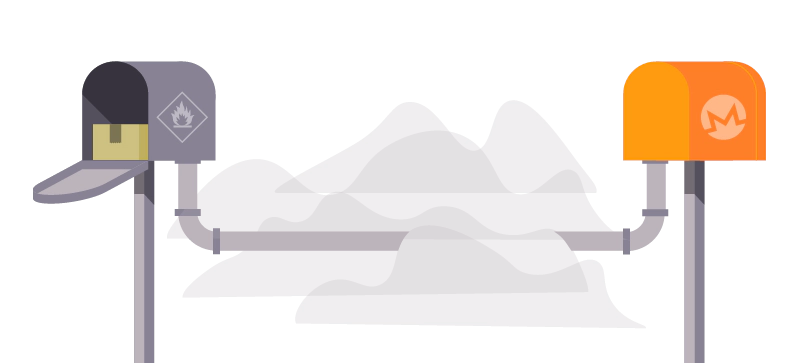
\includegraphics[width=0.5\textwidth]{./images/stealth_address.png}
        \caption{Connessione nascosta tra gli Stealth Address e i wallet}
        \label{fig:encription}
    \end{figure}

    Il team di Buterin ha progettato un sistema di indirizzi nascosti (anche
    detto SAP \footnote{Stealth Address Protocol}) chiamato BaseSAP. Il
    protocollo mira a fornire un meccanismo leggero che consenta agli utenti di
    generare indirizzi invisibili, mantenendo la completa compatibilità con le
    versioni precedenti e non richiedendo modifiche alla blockchain principale.
    BaseSAP è basato sul cifrario assimetrico su curve ellittiche Secp256k1,
    migliorato attraverso l'integrazione di "tags di visualizzazione" utili a
    rendere più efficiente l'analisi rispetto ai comuni DKSAPs
    \footnote{Dual-Key Stealth Address Protocols}.

    Questo protocolli sono la base per le implementazioni DKSAP usate in Monero.
    Da quando DKSAP è nato, ha portato molti ricercatori a studiare e trovare
    nuovi modi per migliorarlo:

    \begin{figure}[ht]
        \centering
        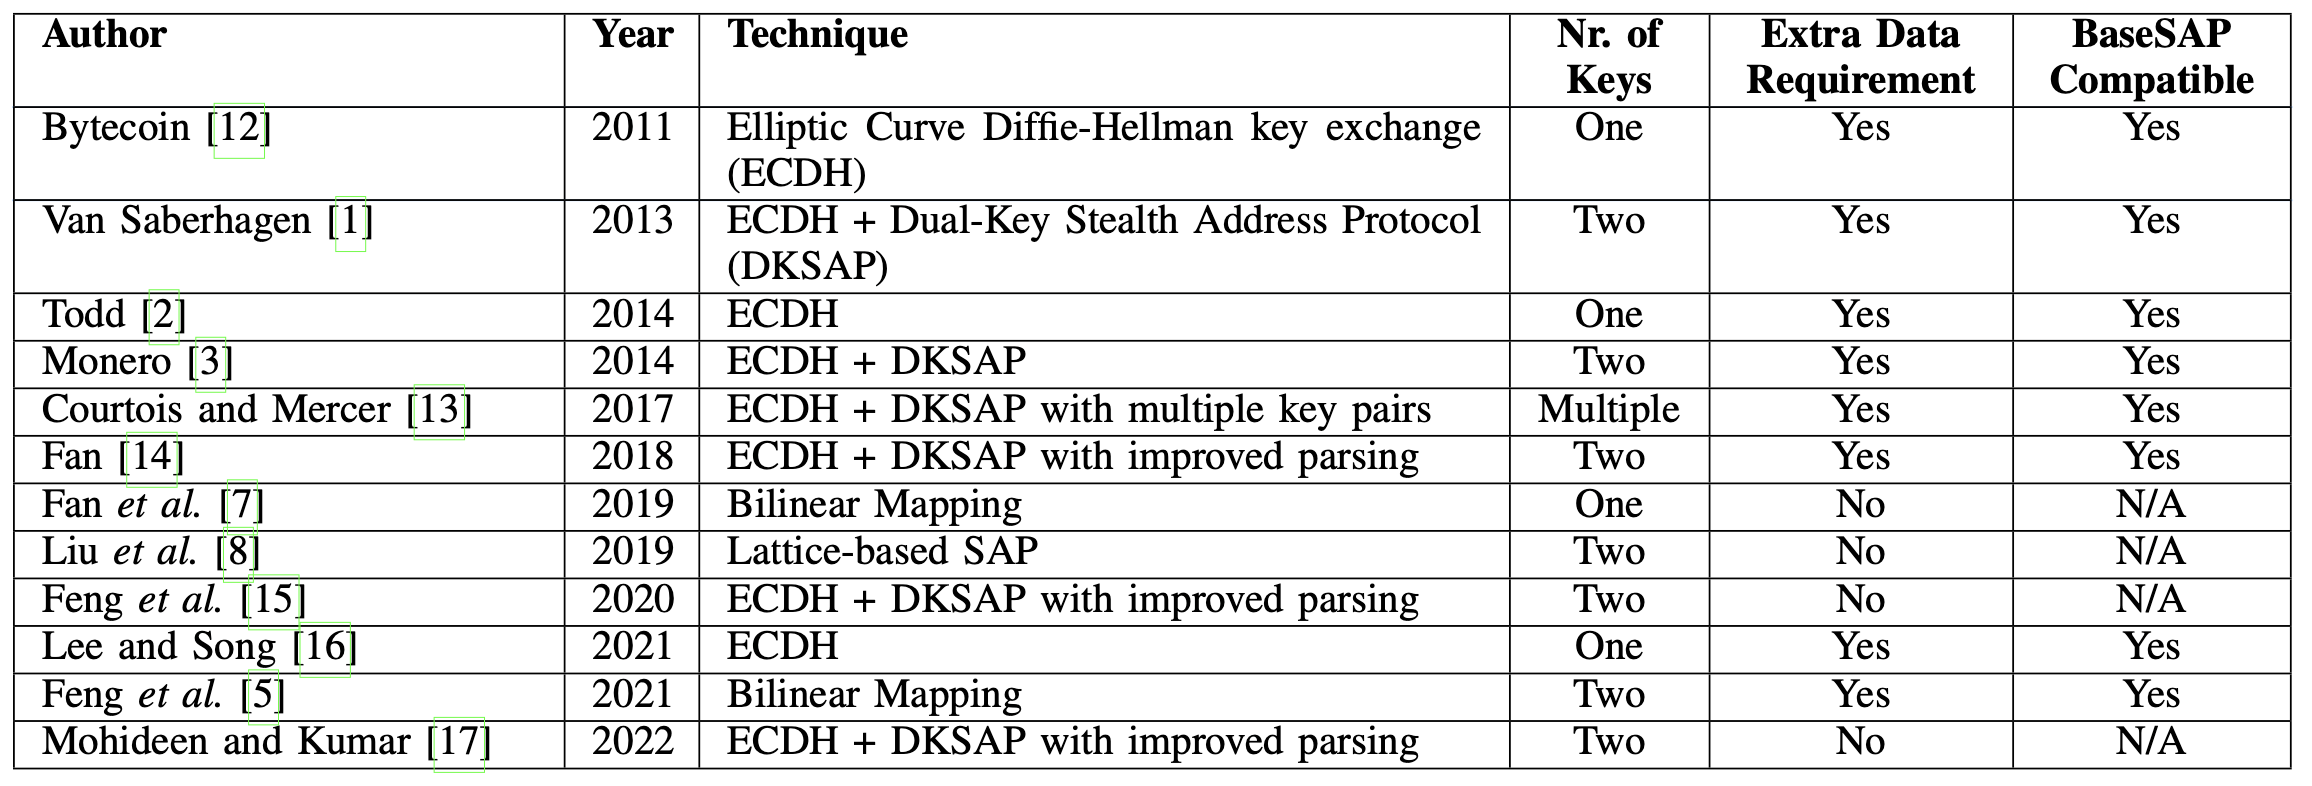
\includegraphics[width=0.95\textwidth]{./images/sommario.png}
        \caption{Sommario dei lavori di ricerca sulle Stealth Address e compatibilità BaseSAP}
        \label{fig:summary}
    \end{figure}



\subsubsection{Ring Signature}

\section{Popolarità}
La popolarità è dovuta al potenziale guadagno, guadagno molto facile da crearsi
poiché per definizoione il cryptojacking punta a sfruttare risorse in possesso
di altri in modo gratuito. Così, anche considerando la volatilità delle cripto
valute, esempio principe BitCoin, i margini di guadagno sono abbastanza alti da
rendere il crimine un vero e proprio business. 

\section{Prevenire e individuare}

\section{Casi reali}

\section{Bibliografia}
\begin{thebibliography}{9}

\bibitem{CSO}
\href{https://arc.net/l/quote/karbftmg}{Cryptojacking explained, CSO}
% \texttt{31-07-2024 15:00}

\bibitem{Botnet}
\href{https://arc.net/l/quote/ftyxgxms}{Botnet, Wikipedia}
% \texttt{31-07-2024 13:00}

\bibitem{zero-day}
\href{https://arc.net/l/quote/golshtco}{2021 Microsoft Exchange Server data breach, Wikipedia}
% \texttt{01-08-2024 16:00}

\bibitem{Monero}
\href{https://arc.net/l/quote/jffmkeln}{Monero, Wikipedia}
% \texttt{01-08-2024 16:30}

\bibitem{FMW}
\href{https://arc.net/l/quote/kbarlqni}{Fileless malware, IEEE Xplore}

\bibitem{Buterin Quote}
Valerio Diaco, \href{https://arc.net/l/quote/qirrmtbh}{\textit{Conosci gli
Stealth Address per star lontano dai radar?}}, Rypto.it, 15 Lugio 2023

\bibitem{BaseSAP}
Anton Wahrstatter , Matthew Solomon, Ben DiFrancesco, Vitalik Buterin, and Davor
Svetinovic \textit{BaseSAP: Modular Stealth Address Protocol for Programmable
Blockchains}, JOURNAL OF LATEX CLASS FILES, VOL. 14, NO. 8, AUGUST 2021, pp. 1–6

\bibitem{Zero To Monero}
Koe, Kurt M. Alonso, Sarang Noether, \textit{A technical guide to a private
digital currency; for beginners, amateurs, and experts} April 4, 2020 (v2.0.0)


\end{thebibliography}


\end{document}